\documentclass[12pt, twoside]{article}
\usepackage[letterpaper, margin=1in, headsep=0.5in]{geometry}
\usepackage[english]{babel}
\usepackage[utf8]{inputenc}
\usepackage{amsmath}
\usepackage{amsfonts}
\usepackage{amssymb}
\usepackage{tikz}
\usetikzlibrary{quotes, angles}
\usepackage{graphicx}
%\usepackage{pgfplots}
%\pgfplotsset{width=10cm,compat=1.9}
%\usepgfplotslibrary{statistics}
%\usepackage{pgfplotstable}
%\usepackage{tkz-fct}
%\usepackage{venndiagram}
\usepackage{multicol}


\usepackage{fancyhdr}
\pagestyle{fancy}
\fancyhf{}
\fancyhead[RE]{\thepage}
\fancyhead[RO]{\thepage \\Name: \hspace{4cm} \, \\}
\fancyhead[LO]{BECA / Dr. Huson / Geometry 10th Grade\\* Unit 5: Transformation, dilation, and scale \\ 22 November 2019}

\renewcommand{\headrulewidth}{0pt}

\begin{document}
\subsubsection*{5.11 Exam: Transformational Geometry}
  \begin{enumerate}

  \begin{multicols}{2}
    [\item A translation maps triangle $PQR$ onto triangle $STU$.] \vspace{0.5cm}
      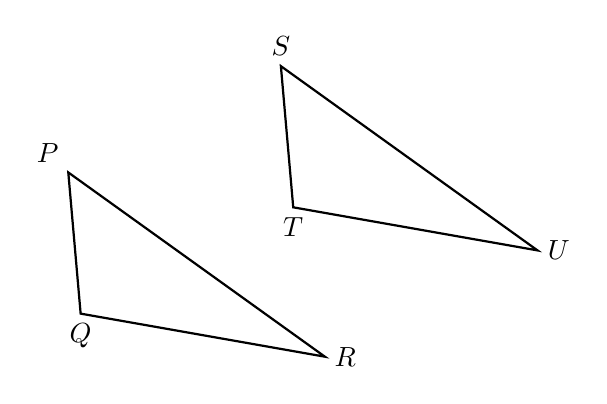
\begin{tikzpicture}[scale=0.9]
        \coordinate [label=above left:$P$](A) at (95:2);
        \coordinate [label=below:$Q$](B) at (0, 0);
        \coordinate [label=right:$R$](C) at (-10:3.5);
        \draw [thick] (A)--(B)--(C)--cycle;
  
        \draw [thick, xshift=3cm, yshift=1.5cm] (95:2) node[above]{$S$}--
        (0,0) node[below]{$T$}--
        (-10:3.5) node[right]{$U$}--cycle;
      \end{tikzpicture}\\
      Write each corresponding object.
      \begin{enumerate}
        \item $Q \rightarrow$ \rule{2cm}{0.15mm}
        \item $\angle QRP \cong$ \rule{2cm}{0.15mm}
        \item \rule{2cm}{0.15mm} $\cong \overline {ST}$
        \item Justify $\triangle PQR \cong \triangle STU$. Use the words ``rigid motion".
      \end{enumerate}
    \end{multicols}  \vspace{1cm}
  
  \item Triangle $ABC$ is dilated with a scale factor of $k$ centered at $A$, yielding $\triangle ADE$, as shown. Given $AB=8$, $BC=10$, $AC=12$, and $DE=15$. \\[0.25cm] Find $AD$, $CE$, and $k$ (the scale factor).
  \begin{flushright}
      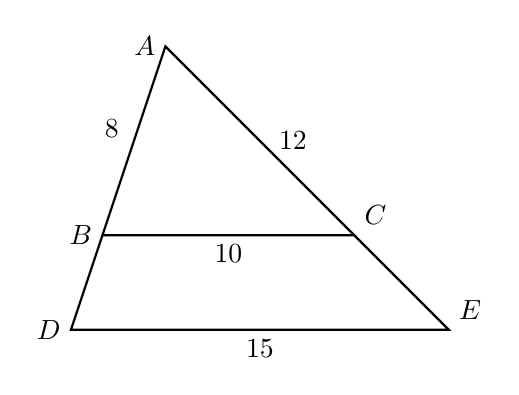
\begin{tikzpicture}[scale=0.4]
        \draw [thick]
        (0,0)node[left]{$B$}--
        (8,0)node[above right]{$C$}--
        (2,6)node[left]{$A$}--cycle;
        \draw [thick]
        (0,0)--
        (-1,-3)node[left]{$D$}--
        (11,-3)node[above right]{$E$}--(8,0);
        \node at (4,0)[below]{$10$};
        \node at (5.3, 3)[right]{$12$};
        \node at (0.3, 2.8)[above]{$8$};
        \node at (5,-3)[below]{$15$};
      \end{tikzpicture}
    \end{flushright}

  \item Translate $\triangle ABC$ by $(x,y) \rightarrow (x+3, y+4)$. Make a table of the coordinates and plot and label the image on the axes.
  \begin{flushright}
      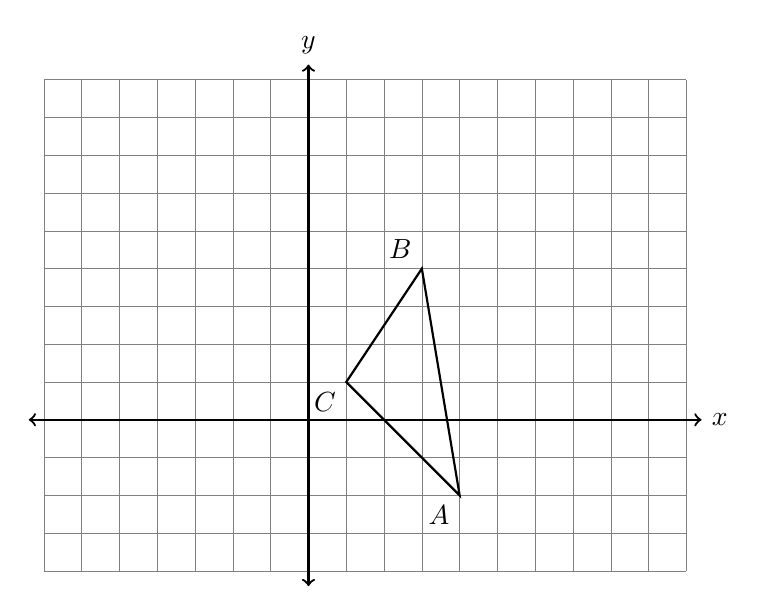
\begin{tikzpicture}[scale=.48]
      \draw [help lines] (-7,-4) grid (10,9);
      \draw [thick, <->] (-7.4,0) -- (10.4,0) node [right] {$x$};
      \draw [thick, <->] (0,-4.4)--(0,9.4) node [above] {$y$};  
      \draw [thick]
        (4,-2) node[below left] {$A$}--
        (3,4) node[above left] {$B$}--
        (1,1) node[below left] {$C$}--cycle;  
    \end{tikzpicture}
  \end{flushright}

  \item A rotation of $90^\circ$ is applied to $\triangle ABC$, mapping it onto $\triangle PQR$, as shown.  \\[0.25cm]
  Which triangle has the larger area, or are they equal? Justify your answer.\\
      \begin{tikzpicture}[scale=.48]
        \draw [thick, <->] (-7.4,0) -- (10.4,0) node [right] {$x$};
        \draw [thick, <->] (0,-5.4)--(0,10.4) node [above] {$y$};
 
        \draw [thick]
        (4,-2) node[below left] {$A$}--
        (8,2) node[right] {$B$}--
        (1,1) node[above right] {$C$}--cycle;
 
        \draw [thick]
        (2,4) node[right] {$P$}--
        (-2,8) node[above] {$Q$}--
        (-1,1) node[below left] {$R$}--cycle;
 
      \end{tikzpicture}
 
  \item Given $\triangle ABP \sim \triangle JKP$ as shown below. $\overline{AB} \parallel \overline{JK}$. $AP=5.7$, $JP=11.4$, and $JK=14.8$. Find $AB$.
  \begin{flushright}
    \begin{tikzpicture}[scale=1.4]
        \draw [thick]
          (0.25,-1)node[right]{$B$}--
          (-0.5,2)node[left]{$K$}--
          (4,0)node[right]{$J$}--
          (0,0)node[above right]{$P$}--
          (-2,0)node[left]{$A$}--cycle;
      \end{tikzpicture}
      \end{flushright}
      \vspace{2cm}

  \item Find the image of $A(-3,1)$ after the translation $(x,y) \rightarrow (x+4,y-2)$.

  \item Given two parallel lines and a transversal, as shown below.
  \begin{center}
  \begin{tikzpicture}
    \draw [<->, thick] (1,2)--(9,2);
    \draw [<->, thick] (0,0)--(8,0);
    \draw [<->, thick] (4,-1)--(5.5,3);
    \node at (4.5,0.3) [left]{$5$};
    \node at (4.5,0.3) [right]{$6$};
    \node at (4.3,-0.3) [left]{$7$};
    \node at (4.3,-0.3) [right]{$8$};
    \node at (5.2,2) [above left]{$1$};
    \node at (5.2,2) [above right]{$2$};
    \node at (5,2) [below left]{$3$};
    \node at (5,2) [below right]{$4$};
  \end{tikzpicture}
  \end{center}
  \begin{enumerate}
    \item State the angle corresponding with $\angle 6$. \vspace{0.5cm}
    \item What theorem would justify $m\angle 5 + m\angle 6 =180^\circ$? \rule{6cm}{0.15mm} \vspace{0.5cm}
    \item What theorem would justify $m\angle 7 = m\angle 2$? \rule{7cm}{0.15mm} \vspace{0.5cm}
    \item Given $m\angle 3 = 73^\circ$ and $m\angle 5 = (3x-1)^\circ$. Find $x$. \vspace{5cm}
  \end{enumerate}

  \item A translation maps $D(2,4) \rightarrow D'(-3,4)$. What is the image of $E(5,-5)$ under the same translation?  \vspace{3.5cm}
  
  \item Given isosceles $\triangle ABC$ with $\overline{AC} \cong \overline{AB}$, $m\angle A = x$, $m\angle B = 55$, and $m\angle C=y$. Find $x$ and $y$. \hfill (\emph{the diagram is not to scale})
  \begin{flushright}
  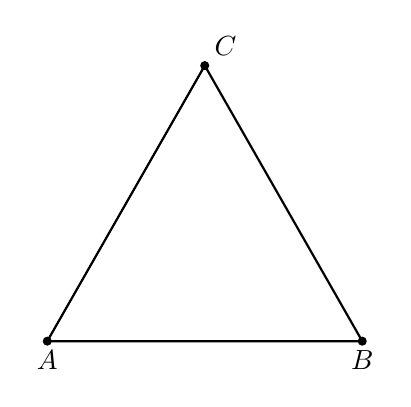
\begin{tikzpicture}[scale=1]
    \draw [thick](0,0)--(4,0)--(2,3.5)--(0,0);
    \draw [fill] (0,0) circle [radius=0.05] node[below]{$A$};
    \draw [fill] (4,0) circle [radius=0.05] node[below]{$B$};
    \draw [fill] (2,3.5) circle [radius=0.05] node[above right]{$C$};
  \end{tikzpicture}
  \end{flushright}

  \item The trapezoid $ABCD$, shown below, undergoes a rigid transformation carrying it onto trapezoid $WXYZ$. State the transformation. (be specific)\\
  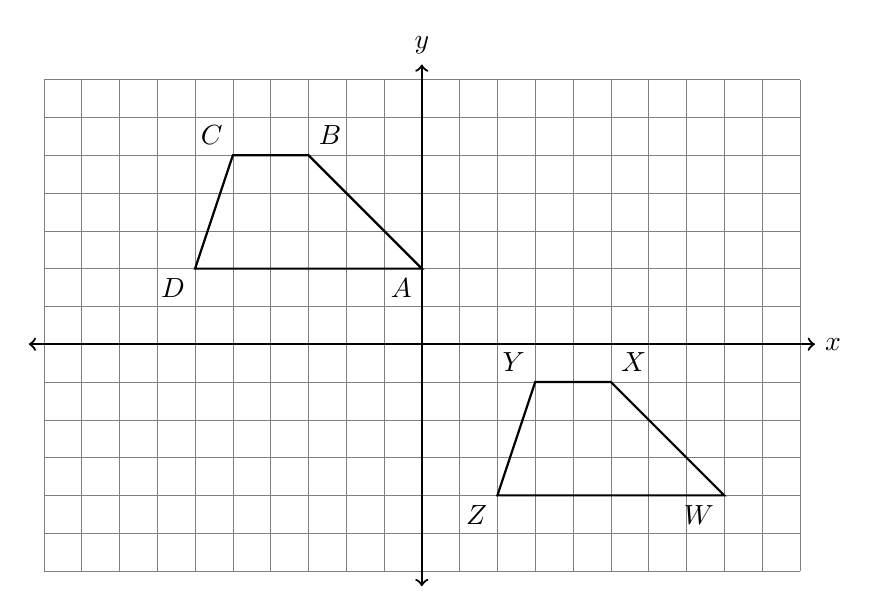
\begin{tikzpicture}[scale=.48]
    \draw [help lines] (-10,-6) grid (10,7);
    \draw [thick, <->] (-10.4,0) -- (10.4,0) node [right] {$x$};
    \draw [thick, <->] (0,-6.4)--(0,7.4) node [above] {$y$};
    \draw [thick]
      (2,-4) node[below left] {$Z$}--
      (3,-1) node[above left] {$Y$}--
      (5,-1) node[above right] {$X$}--
      (8,-4) node[below left] {$W$}--cycle;
    \draw [thick]
      (0,2) node[below left] {$A$}--
      (-3,5) node[above right] {$B$}--
      (-5,5) node[above left] {$C$}--
      (-6,2) node[below left] {$D$}--cycle;
  \end{tikzpicture}

  \item The image of triangle $ABC$ after a rotation is $\triangle A'B'C'$. Is the area of the triangle greater, smaller, or the same after the transformation? Justify your answer. \vspace{3.5cm}

  \item In the diagram below, $\triangle ABC$ with sides of 13, 15, and 16, is mapped onto $\triangle DEF$ after a clockwise rotation of $90^\circ$ about point $P$. \\*[0.25cm]
  If $DE=2x-1$, what is the value of $x$? 
      \begin{flushright}
        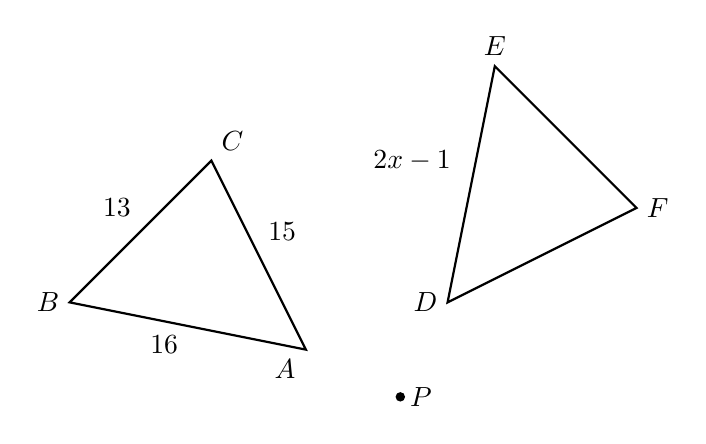
\begin{tikzpicture}[scale=.6]
          %\draw [thick, <->] (-7.4,0) -- (10.4,0) node [right] {$x$};
          %draw [thick, <->] (0,-5.4)--(0,10.4) node [above] {$y$};
          \fill (0,0) circle[radius=0.1] node[right]{$P$};
          \draw [thick]
            (-2,1) node[below left] {$A$}--
            (-7,2) node[left] {$B$}--
            (-4,5) node[above right] {$C$}--cycle;
            \node at (-5,1.5)[below]{16};
            \node at (-6,4){13};
            \node at (-2.5,3.5){15};
            \node at (0.25,5){$2x-1$};
          \draw [thick]
            (1,2) node[left] {$D$}--
            (2,7) node[above] {$E$}--
            (5,4) node[right] {$F$}--cycle;
        \end{tikzpicture}
      \end{flushright}
    \vspace{2cm}

  \item In right triangle $ABC$ shown below, point $D$ is on $\overline{AB}$ and point $E$ is on $\overline{BC}$ such that $\triangle ABC \sim \triangle DBE$. \\*[0.25cm]
  If $AB=15$, $BC=12$, and $EC=7$, what is the length of $\overline{BD}$?
    \begin{flushright}
      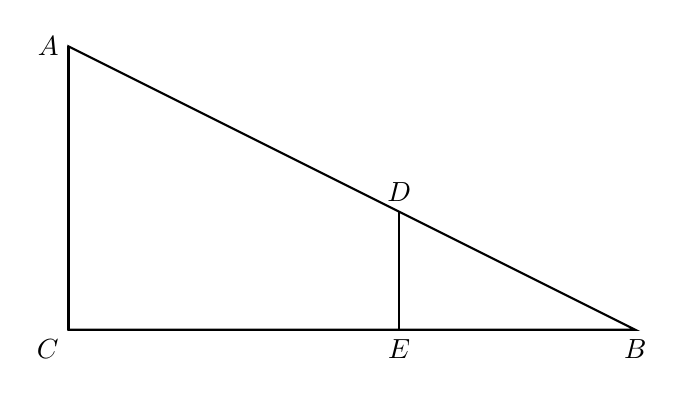
\begin{tikzpicture}[scale=0.6]
        \coordinate [label=left:$A$](A) at (-12,6);
        \coordinate [label=below:$B$](B) at (0, 0);
        \coordinate [label=below left:$C$](C) at (-12,0);
        \coordinate [label=above:$D$](D) at (-5, 2.5);
        \coordinate [label=below:$E$](E) at (-5,0);
        \draw [thick] (A)--(B)--(C)--cycle;
        \draw [thick] (A)--(C);
        \draw [thick] (D)--(E);
      \end{tikzpicture}
    \end{flushright}
  
  \item Given isosceles $\triangle RSU$ with $\overline{UR} \cong \overline{RS}$. If $m\angle UST=140$ find $m\angle U$.
  \begin{flushright}
  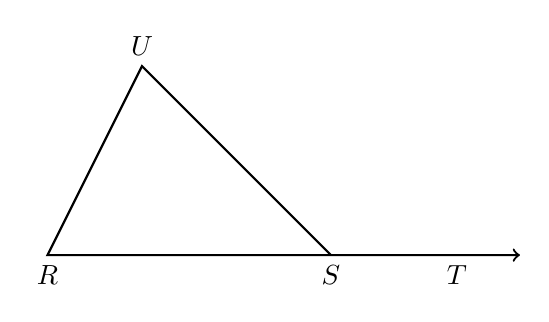
\begin{tikzpicture}[scale=0.8]
    %\draw [->, thick] (0,0)--(5,5);
    \draw [<-, thick] (8,0)--
      (7,0) node[below]{$T$}--
      (0.5,0) node[below]{$R$}--
      (2,3) node[above]{$U$}--
      (5,0) node[below]{$S$};
  \end{tikzpicture}
  \end{flushright} \vspace{1cm}

  \item An angle bisector is shown below, with $\overrightarrow{AC}$ bisecting $\angle BAD$. Given $m\angle BAC = 6x-5$ and $m\angle BAD = 9x+17$, find $m\angle BAD$. (Show check)
  \begin{flushright}
  \begin{tikzpicture}[scale=0.7, rotate=30]
    \draw [<->, thick] (100:7)node[left]{$B$} 
    --(0,0)node[below]{$A$}
    --(6,0)node[below]{$D$}--(7,0);
    \draw [->, thick] (0,0)--(50:7)node[below right]{$C$};
    %\draw [fill] (0,0) circle [radius=0.05] node[below]{$A$};
    %\draw [fill] (5,0) circle [radius=0.05] node[below]{$B$};
  \end{tikzpicture}
  \end{flushright} \vspace{3cm}

  \item The triangle $ABC$, shown below, undergoes two rigid motions carrying it onto triangle $XYZ$. State the two isometric transformations. (be specific)
    \begin{flushright}
      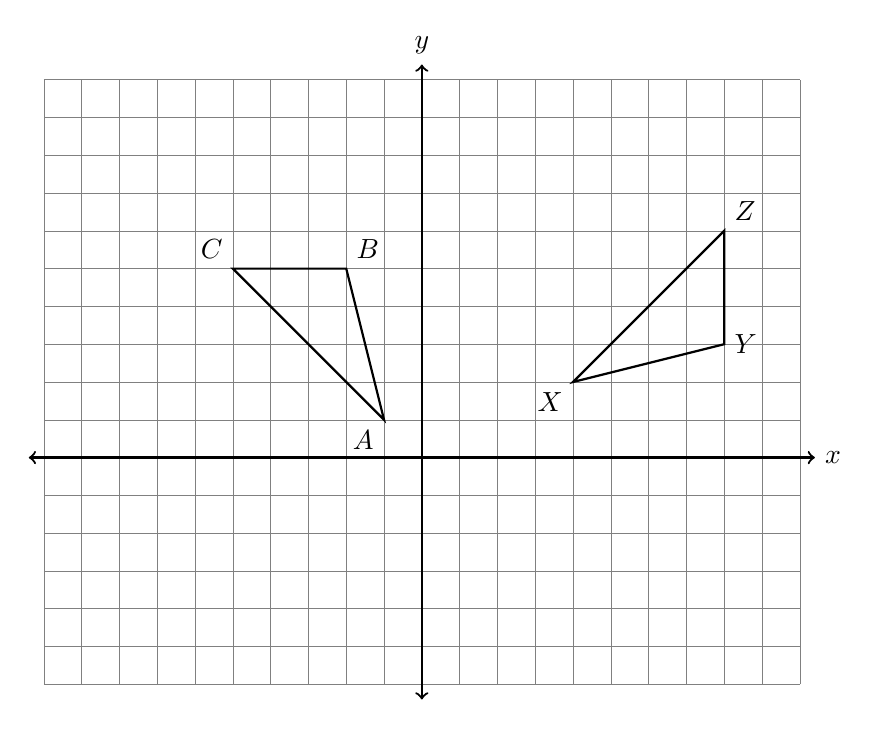
\begin{tikzpicture}[scale=.48]
        \draw [help lines] (-10,-6) grid (10,10);
        \draw [thick, <->] (-10.4,0) -- (10.4,0) node [right] {$x$};
        \draw [thick, <->] (0,-6.4)--(0,10.4) node [above] {$y$};
        \draw [thick]
          (4,2) node[below left] {$X$}--
          (8,3) node[right] {$Y$}--
          (8,6) node[above right] {$Z$}--cycle;
        \draw [thick]
          (-1,1) node[below left] {$A$}--
          (-2,5) node[above right] {$B$}--
          (-5,5) node[above left] {$C$}--cycle;
      \end{tikzpicture}
    \end{flushright}

\item Triangle $\triangle ABC$ is graphed on the set of axes below. The vertices of $\triangle ABC$ have the coordinates $A(2,-3)$, $B(8,1)$, and $C(-1,8)$. \\*[0.25cm]
Reflect the triangle across the $y$-axis. Write down its coordinates in a table and plot and label it on the graph.
    \begin{flushright} %4 quadrant regents grid
    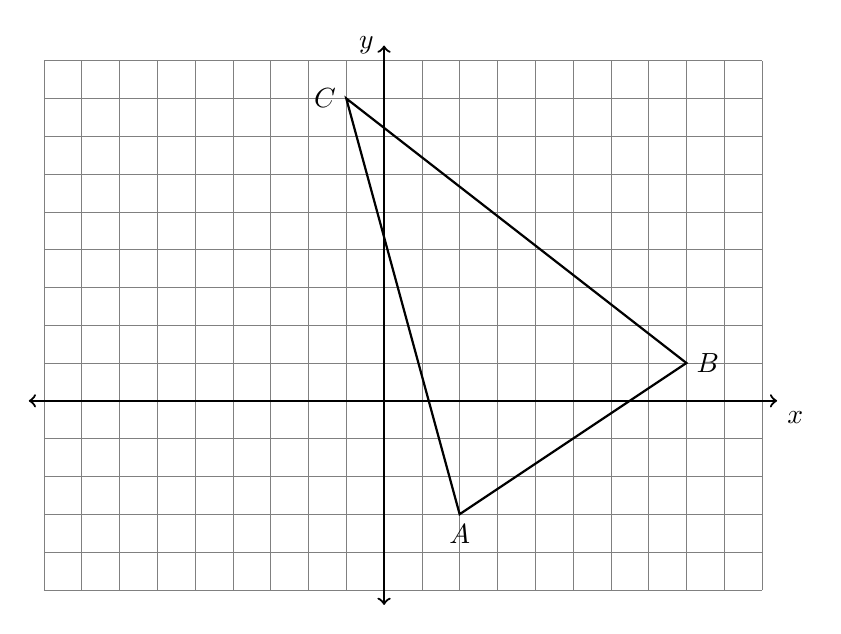
\begin{tikzpicture}[scale=.48]
      \draw [help lines] (-9,-5) grid (10,9);
      \draw [thick, <->] (-9.4,0) -- (10.4,0) node [below right] {$x$};
      \draw [thick, <->] (0,-5.4)--(0,9.4) node [left] {$y$};
      \draw [thick] (2,-3) node[below] {$A$}--
      (8,1) node[right] {$B$}--
      (-1,8) node[left] {$C$}--
      cycle;
      %\draw [fill] (5,0) circle [radius=0.1] node[above left] {$P$};
    \end{tikzpicture}
    \end{flushright}
    
  \item Given parallel lines $\overleftrightarrow{AB} \parallel \overleftrightarrow{CDE}$ with $\overline{AC} \cong \overline{AD}$. If $m\angle BAD=70$ find $m\angle ACD$.
    \begin{flushright}
    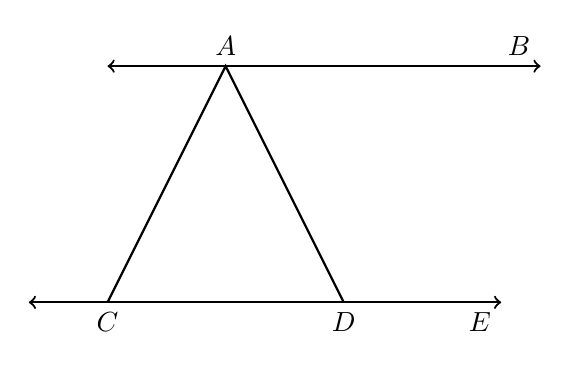
\begin{tikzpicture}
      \draw [<->, thick] (1,3)--(6.5,3) node[above left]{$B$};
      \draw [<->, thick] (0,0)--
        (5,0)--
        (6,0) node[below left]{$E$};
      \draw [-, thick] (1,0) node[below]{$C$}--
        (2.5,3) node[above]{$A$}--
        (4,0) node[below]{$D$};
    \end{tikzpicture}
    \end{flushright} \vspace{1.5cm}

\newpage
\subsubsection*{Early finishers}

  \item Of two complementary angles, the measure of $\angle A$ is two times that of $\angle B$. Find $m\angle A$. \vspace{3.5cm} 


  \item In  $\triangle ABC$ shown below, side $\overline{AC}$ is extended to point $D$ with $m\angle DAB=(6x-16)^\circ$, $m\angle C=(x+4)^\circ$, and $m\angle B=(4x+3)^\circ$. \\[0.25cm]
  What is $m\angle BAC$?
  \begin{flushright}
      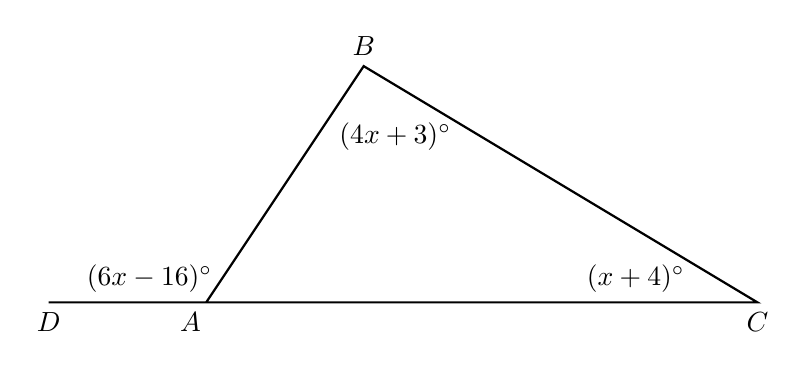
\begin{tikzpicture}
        \draw [thick](0,0)node[below]{$D$}--
          (1.8,0)node[below]{$A$}--
          (9,0)node[below]{$C$}--
          (4,3)node[above]{$B$} --(2,0);
          \node at (2.2,0)[above left]{$(6x-16)^\circ$};
          \node at (8.2,0)[above left]{$(x+4)^\circ$};
          \node at (4.4,2.4)[below]{$(4x+3)^\circ$};
      \end{tikzpicture}
    \end{flushright}

  \item Triangle $ADE$ and its midline $\overline{BC}$ are drawn, with $B$ the midpoint of $\overline{AD}$ and $C$ the midpoint of $\overline{AE}$. The two medians $\overline{AE}$ and $\overline{AE}$ are drawn, as shown, intersecting in point $F$, the centroid.\\[0.25cm]
  $\triangle FCB \sim \triangle FDE$ with scale factor $k=2$.\\[0.25cm]
  Given $BC=7$, find $DE$. \\[0.25cm] Given $BF=4$, find $FE$. %\vspace{1cm}
  \begin{flushright}
      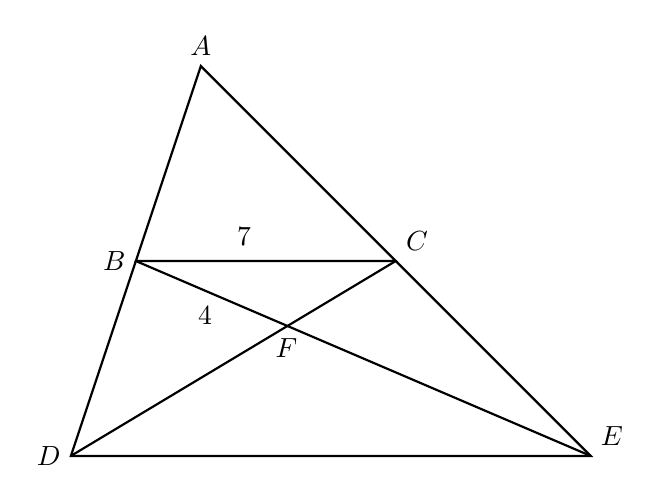
\begin{tikzpicture}[scale=0.55]
        \draw [thick]
        (0.5,1.5)node[left]{$B$}--
        (6.5,1.5)node[above right]{$C$}--
        (2,6)node[above]{$A$}--cycle;
        \draw [thick]
        (0.5,1.5)--
        (-1,-3)node[left]{$D$}--
        (11,-3)node[above right]{$E$}--(6.5,1.5);
        \draw [thick] (0.5,1.5)--(11,-3);
        \draw [thick] (6.5,1.5)--(-1,-3);
        \node at (3,2.5)[below]{$7$};
        \node at (3.5, -0.5)[right]{$F$};
        \node at (2.1, -0.2)[above]{$4$};
        %\node at (-0.7, -1)[above]{$5$};
      \end{tikzpicture}
    \end{flushright} \vspace{1cm}

  \item On the set of axes below, $\triangle ABC$ has vertices at $A(-2,0)$, $B(2,4)$, $C(4,-2)$, and $\triangle DEF$ has vertices at $D(4,0)$, $E(-4,8)$, $F(-8,-4)$.
  \begin{center}
    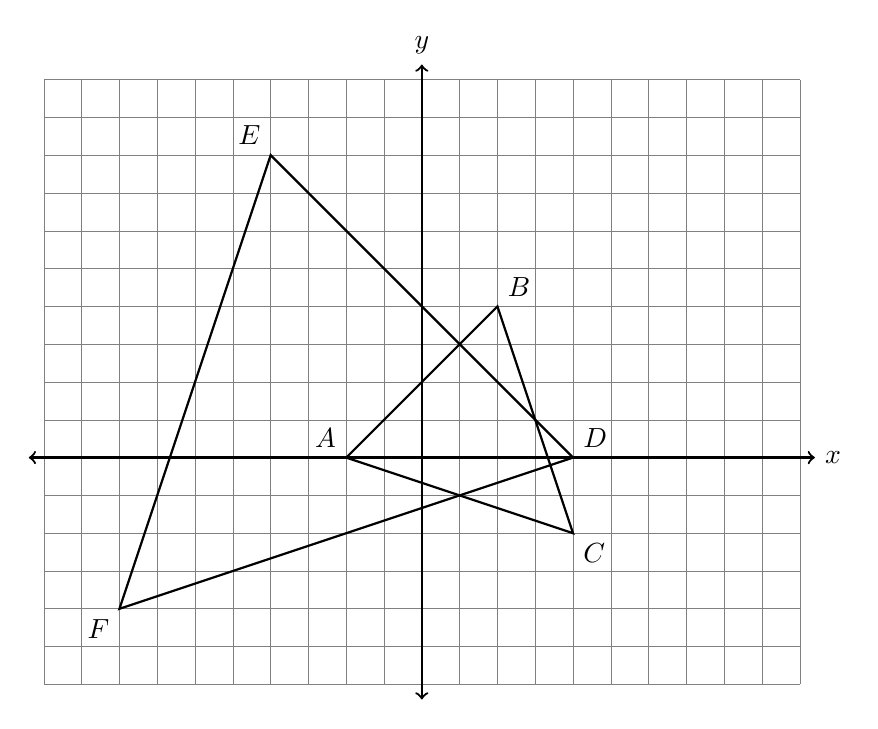
\begin{tikzpicture}[scale=.48]
      \draw [help lines] (-10,-6) grid (10,10);
      \draw [thick, <->] (-10.4,0) -- (10.4,0) node [right] {$x$};
      \draw [thick, <->] (0,-6.4)--(0,10.4) node [above] {$y$};
      \draw [thick]
        (-2,0) node[above left] {$A$}--
        (2,4) node[above right] {$B$}--
        (4,-2) node[below right] {$C$}--cycle;
      \draw [thick]
        (4,0) node[above right] {$D$}--
        (-4,8) node[above left] {$E$}--
        (-8,-4) node[below left] {$F$}--cycle;
    \end{tikzpicture}
  \end{center}
  Which tranformations map $\triangle ABC \rightarrow \triangle DEF$? Mark each statement True or False
    \begin{enumerate}
      \item A dilation with a scale factor of $-2$ centered at the origin \hfill True \quad False
      \item A dilation with a scale factor of $\frac{1}{2}$ centered at point $A$ \hfill True \quad False
      \item A dilation with a scale factor of 2 centered at the origin, followed by a rotation of $180^\circ$ about the origin \hfill True \quad False
      \item A dilation with a scale factor of 2 centered at the origin, followed by a reflection across the $y$-axis \hfill True \quad False
    \end{enumerate}


\end{enumerate}
\end{document}
